\section{Type of Variable}
\label{sec:concept_diffval}
In Rust, there are three variable types: owner, reference, and slice (only for sequence of values). 
A developer is sometimes forced to use specific variable types. For example, some of methods are only implemented to specific variable types.
However, one can select any variable types for operation in most case.

These variables have different memory representation shown in Figure~\ref{fig:own_ref_slice}.
The owner has a pointer pointing to the memory address of sequence values, length of the values, and capacity allocated to store additional values. 
Reference and Slice are variables borrowing value owned by other variable. The reference is a pointer that points to the owner. 
The slice is a pointer that points to memory address of sequence values. It has value such as length of sequence values stored in the memory. 
Since they have different memory representation, an assumption is that it takes different time to access to the contents of the memory among these pointer types.
We examine this by constructing complex objects whose fields are these variable types. The details are explained in section 3.2.

\begin{figure}[htb]
    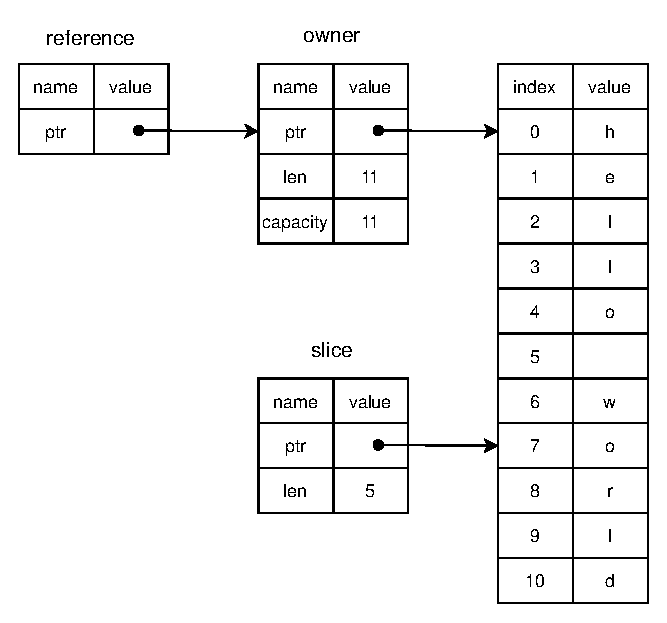
\includegraphics[width=10cm]{own_ref_slice.eps}
    \caption{Memory Representation of Owner, Reference, and Slice Type}
    \label{fig:own_ref_slice}
\end{figure}

\section{Reference Count}
\label{sec:concept_refcount}
Reference is useful to avoid movement of ownership. However, one needs to track its lifetime and explicitly includes it in code, 
because Rust compiler cannot infer it. This can be another encumbrance. We can instead acquire multiple owners to single value by using Reference Counting (Rc). 
By leveraging Rc, a value can be shared like what borrowing plays the role in Rust programming. 

The difference is that Rc checks number of owner pointing to the actual data and makes sure the data is not deleted 
until all the owners are dereferenced. Using Rc is sometimes preferable approach for developers especially when lifetime planning is extremely difficult.
However, the possible problems regarding to Rc are the cost for tracking the number of references and allocating memory on heap instead of stack.
Having these assumption, an experiment is conducted to examine difference of runtime performance of dropping reference and Rc. 
This is explained in section 3.2.

\section{Multithread}
\label{sec:concenpt_multithreading}
In Rust programming, writing concurrent code is relatively easy. The care Rust takes with reference, mutability, and lifetimes is valuable enough in single-threaded programs, 
but it also is in concurrent programming. Rust has tools to write concurrent code, such as threads, locks, atomic reference. 
One can implement various concurrent codes for the same purpose with different memory management strategies. 
The most ubiquitous tool used in Rust concurrent code is Atomic Reference Counting (Arc). 

Arc is a simple interface that allows threads to share data. Arc allows multiple variable to have ownerships of a particular value similarly to Rc, 
but also supports atomic feature enabling the ownerships exist in different threads. 
In many situation where developer write a multithreading code, the deletion of Arc happens significant amount of times. 
Similarly to Rc, our assumption is that deletion of Arc has also overhead when we compare to normal reference. 
To assess runtime performances of algorithm with Arc vs normal reference, we implement merge-sort algorithm in two different ways. 

\section{Tree-aggregate}
\label{sec:concept_treeagg}
Finally, we implement some of algorithm common in Big Data processing. One of them is tree-aggregate.

Tree-aggregate is a communication patten heavily used for Machine Learning algorithm in Spark (MLlib \cite{DBLP:journals/jmlr/MengBYSVLFTAOXX16}). 
The topology of aggregation patterns in Apache Spark are shown in Figure~\ref{fig:aggregationk_patttern}. 
In the traditional aggregation function in Spark, results of aggregation in all executor clusters are sent to the driver. 
That is why this operation suffers from the CPU cost in merging partial results and the network bandwidth limit.
Tree-aggregate is a communication pattern which overcomes these problems by breaking aggregate operation in multi-level represented like tree structure.

Spark generates intermediate objects from RDDs. In Tree-aggregation, aggregated HashMap like data structure is created in each thread or node. 
When it aggregates objects in RDD, copy of objects should be performed to construct intermediate aggregated data structure.
In another possible way that might be implemented, one can use reference to the objects to perform aggregation instead of copying the values themselves.
In Rust, we can clone or get Arc (Rc if in single thread) of objects to implement these operations.

Since Tree-aggregation algorithm generates and deletes a lot of intermediate data structures, 
how the data structures are constructed and how they are deallocated is important concern in memory management in this algorithm.
In our experiment, tree-aggregation algorithms are examined in multi-threading. The detail is described in section 3.2.

\begin{figure}[htb]
    \begin{minipage}[t]{0.5\linewidth}\centering
        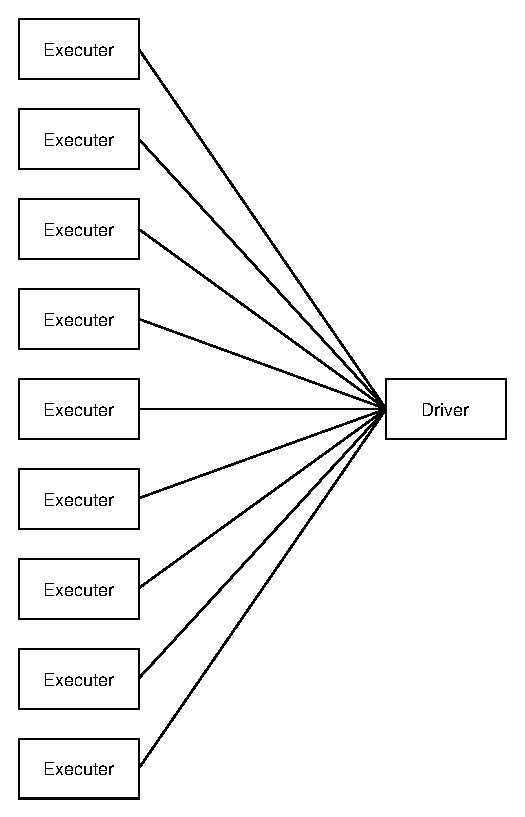
\includegraphics[width=5cm]{normal_agg.eps}
        \medskip
        \centerline{(a)}
        \end{minipage}\hfill
        \begin{minipage}[t]{0.5\linewidth}\centering
        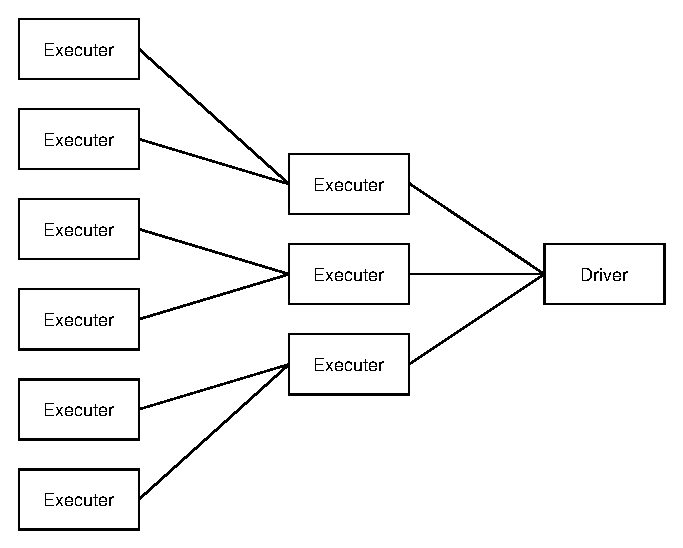
\includegraphics[width=7cm]{tree_agg.eps} 
        \medskip
        \centerline{(b)}
    \end{minipage}\hfill
    \caption{Representation of aggregation strategies in Apache Spark: (a) Traditional Aggregation, (b) Tree Aggregation}
    \label{fig:aggregationk_patttern}
\end{figure}

\section{K-Nearest-Neighbors}
\label{sec:concept_history}
The other algorithm common in Big Data processing is K-nearest-neighbors (KNN). KNN is a traditional Machine Learning algorithm which classify targets into categories. 
In training KNN, it simply stores all available training data without calculation. At prediction phase, targets are given and similarity measures are calculated. 
Based on these similarities, the algorithm selects \(K\) (user-defined number) training observations similar to the each target. 
Then, it checks corresponding categories of the \(K\) observations to determine predicted category. 

In brute force algorithm, KNN calculates similarity measures for all combinations among training and testing observations. 
If training data has \(N\) observations and test data has \(M\) observations, KNN needs to calculate \(N \times M\) similarity measures. 
Sort or binary heap can be used to select the \(K\) most similar training observations.

In our experiment, KNN algorithms performs document classification and implemented in multithread. 
There are three phases in our algorithm: preprocessing, query, and combine phase. 
In preprocessing phase, the algorithm calculates Term-frequencies (Tfs) to generate numeric feature vectors and matrices. 
In query phase, similarity measures are calculated and \(K\) nearest neighbors are selected. 
For similarity measure, our choice is cosine similarity(~\ref{eq:cosine}). 
In combine phase, results of query phase are gathered and combined from each threads.

\begin{equation} \label{eq:cosine}
    Cos(\vec{x}, \vec{t})
     = \frac{\sum_{i=0}^{n} (x_i t_i)}{\sqrt{\sum_{i=0}^{n} x_i^2}\sqrt{\sum_{i=0}^{n} t_i^2}}
\end{equation}

Even though preprocessing phase is not specific process for KNN algorithm, 
it is common in algorithms used in Natural Language Processing. Therefore, better memory management strategy should be applied in this preprocessing phase.
This preprocessing generates many intermediate data structures and copies of String elements are used in these data structure again and again. 
We can again either clone or get Arc of String. 

Our KNN algorithms are implemented with batch processing. In query phase, we control batch size to examine how size of objects allocated simultaneously in memory has impact to algorithm's runtime performance.
The detail implementation is explained in section3.2.

\section{Complex Objects}
\label{sec:concept_history}
To conduct experiments for above concepts, we use the 4 types of complex object: CustomerOwned, CustomerBorrowed, CustomerSlice, and CustomerRc. 
These object contains other type of object: OrderOwned, OrderBorrowed, OrderSlice, and OrderRc.
The representation of these objects are shown in Figure~\ref{fig:customer} and Figure~\ref{fig:order}. 
Three Customer objects have 15 fields: 3 fields for i32, 3 fields for f64, 8 fields for String, and 1 field for Order object.
All of fields of CustomerOwned and OrderOwned are owned by the object. On the other hand, fields of CustomerBorrowed, CustomerSlice, OrderBorrowed, and OrderSlice are borrowed. 
Reference of slice of values are used as the fields and owner of actual values are stored differently in source Vec. 
CustomerRc acquires Rc of values used for its fields from the source Vec.

\begin{figure}[htb]
    \begin{minipage}[t]{0.2\linewidth}\centering
        \begin{lstlisting}
            struct CustomerOwned {
                key: i32,
                age: i32,
                num_purchase: i32,
                total_purchase: f64,
                duration_spent: f64, 
                duration_since: f64,
                zip_code: String,
                address: String,
                country: String,
                state: String,
                first_name: String,
                last_name: String,
                province: String,
                comment: String, 
                order: OrderOwned
            }
        \end{lstlisting}
      \medskip
      \centerline{(a)}
    \end{minipage}\hfill
    \begin{minipage}[t]{0.6\linewidth}\centering
        \begin{lstlisting}
            struct CustomerBorrowed<'a> {
                key: &'a i32,
                age: &'a i32,
                num_purchase: &'a i32,
                total_purchase: &'a f64,
                duration_spent: &'a f64, 
                duration_since: &'a f64,
                zip_code: &'a String,
                address: &'a String,
                country: &'a String,
                state: &'a String,
                first_name: &'a String,
                last_name: &'a String,
                province: &'a String,
                comment: &'a String, 
                order: &'a OrderBorrowed<'a>
            }
        \end{lstlisting}
      \medskip
      \centerline{(b)}
    \end{minipage}
    \begin{minipage}[t]{0.2\linewidth}\centering
        \begin{lstlisting}
            struct CustomerSlice<'a> {
                key: &'a i32,
                age: &'a i32,
                num_purchase: &'a i32,
                total_purchase: &'a f64,
                duration_spent: &'a f64, 
                duration_since: &'a f64,
                zip_code: &'a str,
                address: &'a str,
                country: &'a str, 
                state: &'a str,
                first_name: &'a str,
                last_name: &'a str,
                province: &'a str,
                comment: &'a str,
                order: &'a OrderSlice<'a>
            }
        \end{lstlisting}
      \medskip
      \centerline{(c)}
    \end{minipage}\hfill
    \begin{minipage}[t]{0.6\linewidth}\centering
        \begin{lstlisting}
            struct CustomerRc {
                key: Rc<i32>,
                age: Rc<i32>,
                num_purchase: Rc<i32>,
                total_purchase: Rc<f64>,
                duration_spent: Rc<f64>,
                duration_since: Rc<f64>,
                zip_code: Rc<String>,
                address: Rc<String>,
                country: Rc<String>,
                state: Rc<String>,
                first_name: Rc<String>,
                last_name: Rc<String>,
                province: Rc<String>,
                comment: Rc<String>,
                order: Rc<OrderRc>
            }
        \end{lstlisting}
      \medskip
      \centerline{(c)}
    \end{minipage}\hfill
    \caption{Representation of Customer objects Whose fields are different variable type: (a) CustomerOwned struct whose fields are all owned 
    (b) CustomerBorrowed struct whose fields are borrowed with reference (c) CustomerSlice struct whose fields are borrowed with slice for sequence value, otherwise reference}
    \label{fig:customer}
 \end{figure}

 \begin{figure}[htb]
    \begin{minipage}[t]{0.2\linewidth}\centering
        \begin{lstlisting}
            struct OrderOwned {
                order_id: i32,
                num_items: i32, 
                payment: f64,
                order_time: f64,
                title: String,
                comment: String
            } 
        \end{lstlisting}
      \medskip
      \centerline{(a)}
    \end{minipage}\hfill
    \begin{minipage}[t]{0.6\linewidth}\centering
        \begin{lstlisting}
            struct OrderBorrowed<'a> {
                order_id: &'a i32,
                num_items: &'a i32, 
                payment: &'a f64,
                order_time: &'a f64,
                title: &'a String,
                comment: &'a String
            }
        \end{lstlisting}
      \medskip
      \centerline{(b)}
    \end{minipage}
    \begin{minipage}[t]{0.2\linewidth}\centering
        \begin{lstlisting}
            struct OrderSlice<'a> {
                order_id: &'a i32,
                num_items: &'a i32, 
                payment: &'a f64,
                order_time: &'a f64,
                title: &'a str,
                comment: &'a str
            }
        \end{lstlisting}
      \medskip
      \centerline{(c)}
    \end{minipage}\hfill
    \begin{minipage}[t]{0.6\linewidth}\centering
        \begin{lstlisting}
            struct OrderRc {
                order_id: Rc<i32>,
                num_items: Rc<i32>,
                payment: Rc<f64>,
                order_time: Rc<f64>,
                title: Rc<String>,
                comment: Rc<String>
            }
        \end{lstlisting}
      \medskip
      \centerline{(c)}
    \end{minipage}\hfill
    \caption{Representation of Order objects Whose fields are different variable type: (a) OrderOwned struct whose fields are all owned 
    (b) OrderBorrowed struct whose fields are borrowed with reference (c) OrderSlice struct whose fields are borrowed with slice for sequence value, otherwise reference}
    \label{fig:order}
 \end{figure}

\clearpage
